
\documentclass[12pt]{article}

% margin left and right with \setlength{\itemindent}{-.5in} %
\usepackage{enumitem}

% leave out section numbers in subsection numbering %
\usepackage[T1]{fontenc}
\renewcommand*\thesubsection{\arabic{subsection}}

% include Roman numerals for sections %
\renewcommand{\thesection}{\Roman{section}}
%Roman numerals for subsections like this \renewcommand{\thesubsection}{\Roman{subsection}}%
% include the pckage of the color%
\usepackage[usenames, dvipsnames]{color}
\usepackage[english]{babel}
\usepackage[utf8x]{inputenc}
\usepackage{amsmath}
\usepackage{graphicx}
\usepackage{subfiles}

%define your own color %
\definecolor{mygray}{gray}{0.9}
\begin{document}
	\listoffigures
	\title{Chapter 3 : Conception}
	\maketitle
	
	\section{Introduction}

	\section{Modeling Language}
		A modeling language is used to describe a system, a standard or methodology, general or domain-specific and / or context based on its components and relationships.
	There are several modeling languages, the best known are UML and Merise. In our project we chose UML as Modeling language.
	\\
	UML is a Unified Modeling language that can can model a problem in a standard way.
	\\
	\\
	\textbf{Why UML ?}
	\\
	\\
	We chose UML for these reasons : 
	\begin{itemize}
	\item To obtain a very high level modeling independent of the language and environments
	\item Document a project. 
	\end{itemize}
	
	\section{Global Conception}
	In this section, we highlight the architecture of our application, we starting  with physical architecture and the logical architecture.
	
	\clearpage
	\newpage
	\subsection{Physical Architecture}
	It is primordial to designing any computer system to choose the model architecture that will be adequate to ensure proper functioning, performance, the reuse and reliable interconnection of this system with others. We opt for this purpose for the physical architecture described in the figure below.
	\begin{figure}[h]
		\centering
		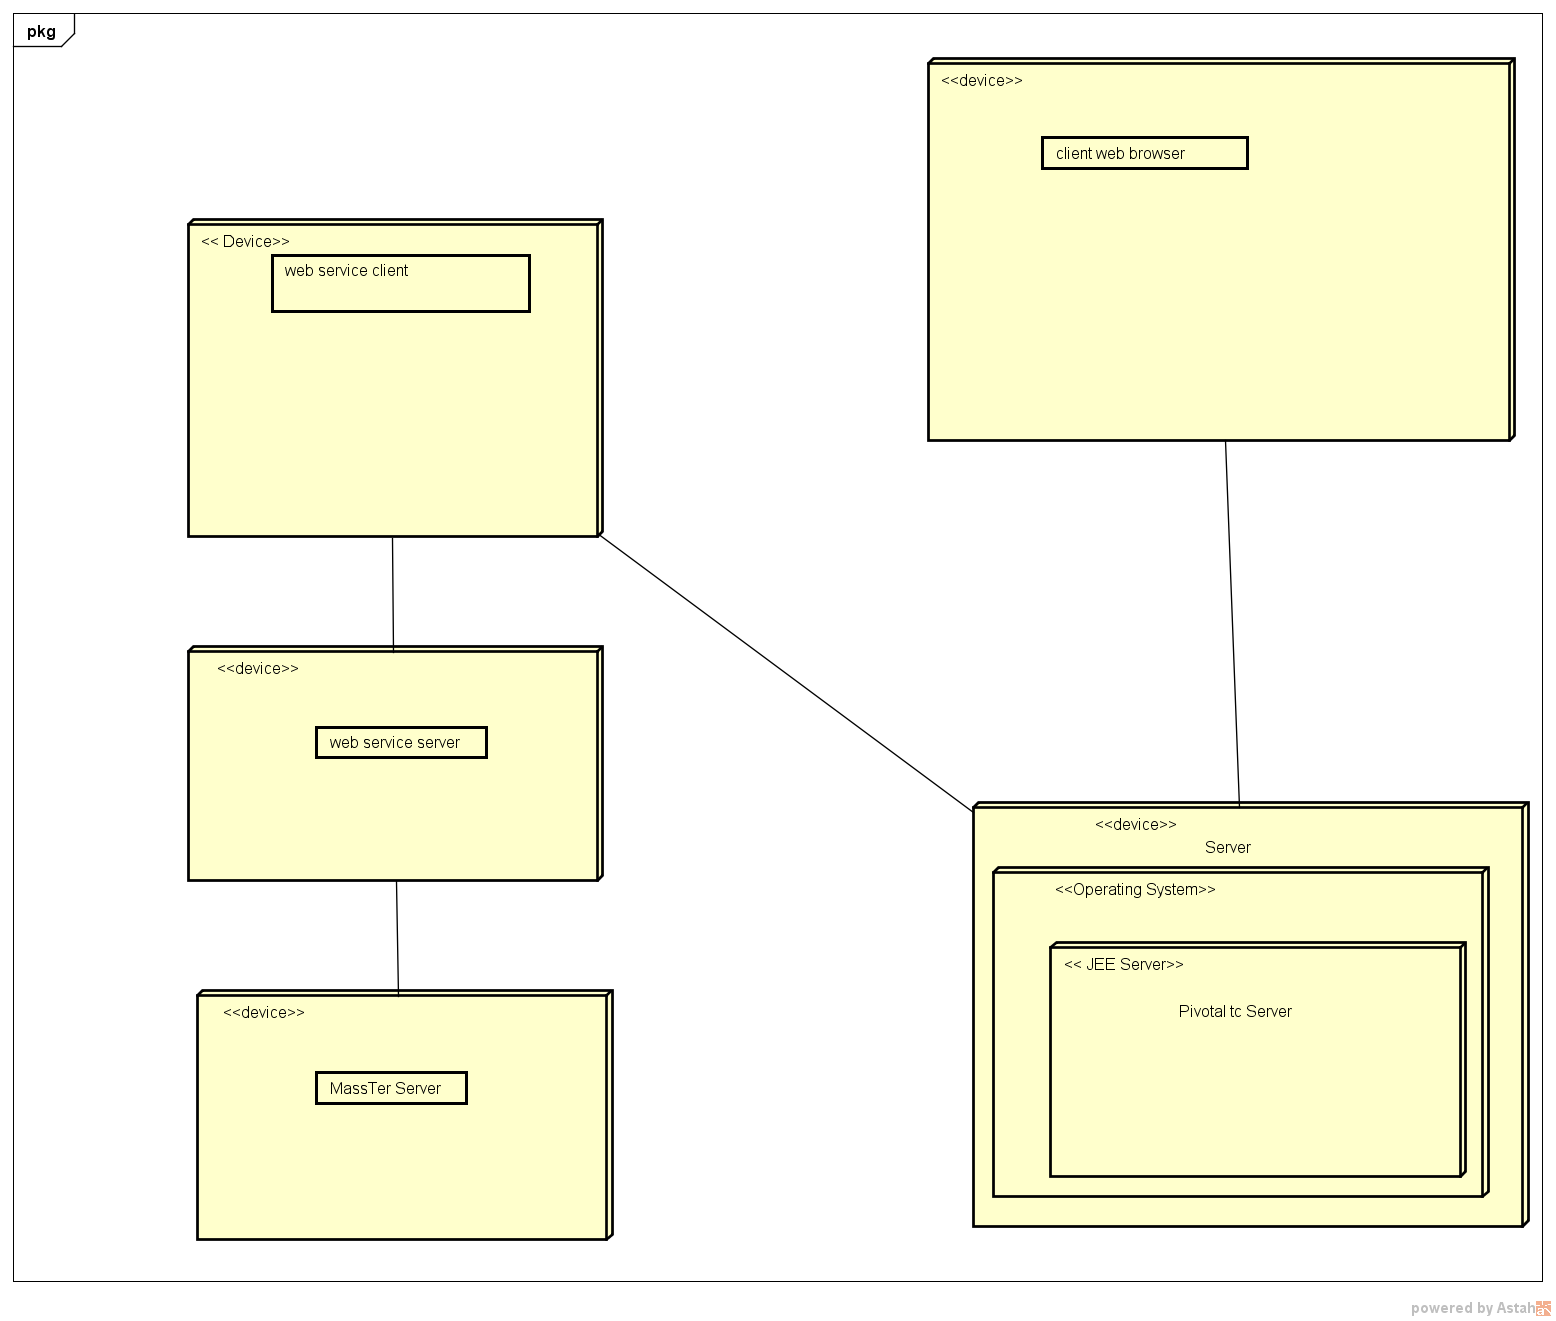
\includegraphics[width=1\textwidth]{DeploymentDiagramPhysicalArchitecture.png}
		\caption{Deployment Diagram Physical Architecture}
	\end{figure}  

	\clearpage
    \newpage  
	
	\subsection{Logical Architecture}
		\begin{figure}[h]
		\centering
		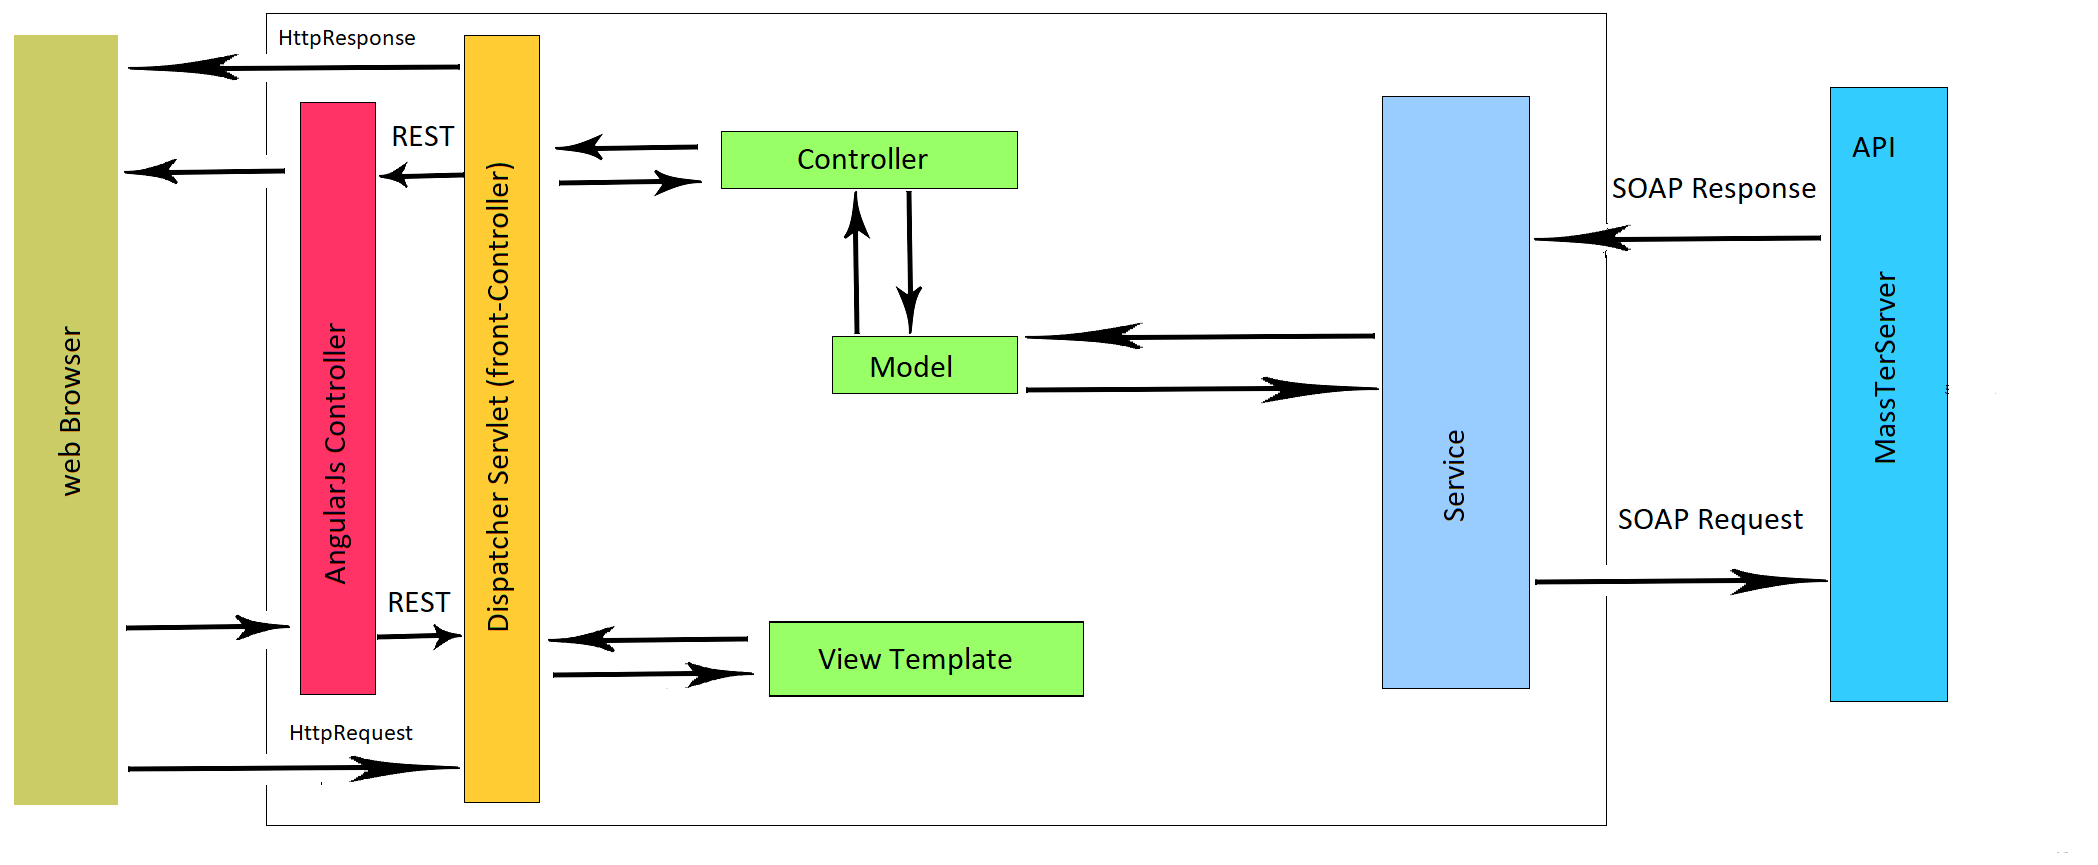
\includegraphics[width=1\textwidth]{logicalArchitecture.png}
		\caption{Logical Architecture}
	\end{figure}  
	

    \clearpage
	\newpage
	\subsection{Design Pattern}
		We opt to use the MVC design pattern for the benefits if offers :
	\begin{itemize}
		\item \textbf{Reliability : }The presentation and business layers are completely separate, so that the business can change without necessarily affecting the presentation, or vice versa.
		\item \textbf{Adaptability : }Any visual representation can be easily integrated.
		\item \textbf{Productivity : }The duration of development is significantly reduced, in allowing parallel work teams.
		\item \textbf{Extensible : } With MVC the code is extensible.
	\end{itemize}

	\clearpage
    \newpage

	\section{Detailed Conception}
    \clearpage
	\newpage
	\subsection{Package Diagram}
		\begin{figure}[h]
		\centering
		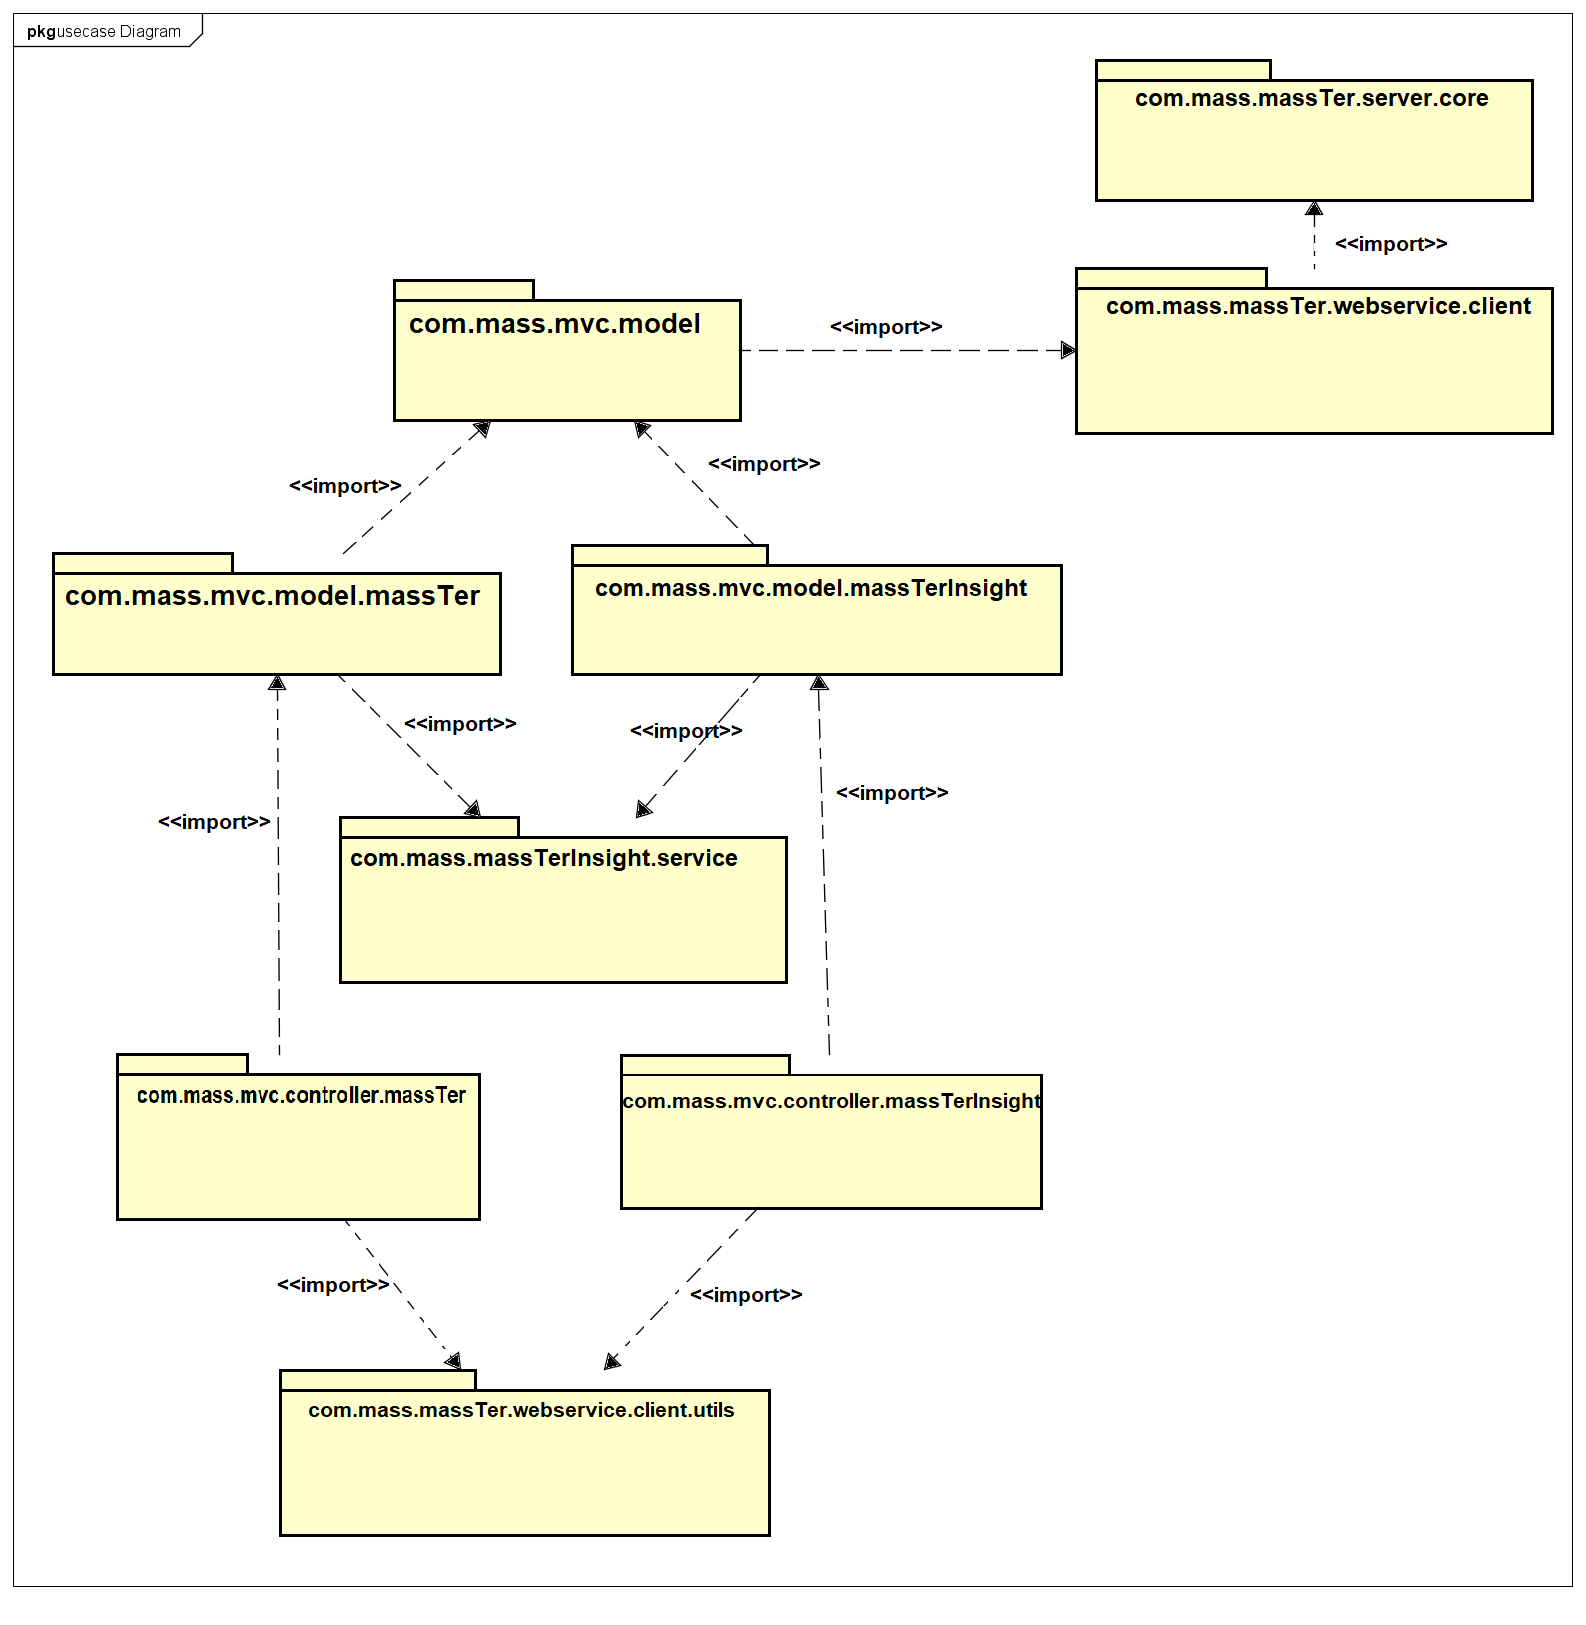
\includegraphics[width=1\textwidth]{packageDiagram.png}
		\caption{package diagram}
	\end{figure}  
	
	\clearpage
	\newpage
	\subsection{Class Diagram}
	\begin{figure}[h]
		\centering
		\includegraphics[width=1\textwidth]{classDiagram.png}
		\caption{Class diagram}
	\end{figure} 
	\clearpage
	\newpage
	\subsection{Sequence Diagram}
	\subsubsection{Sequence Diagram use case ``connect to MassTer Server''}
	The access to all the service of MassTer Insight is shall be preceded by the connection to The MassTer Server (API). All the users (Admin and Data-Analysts) should enter the address and the port of MassTer Sever to benefits from all the services of this API.
	
	\begin{figure}[h]
		\centering
		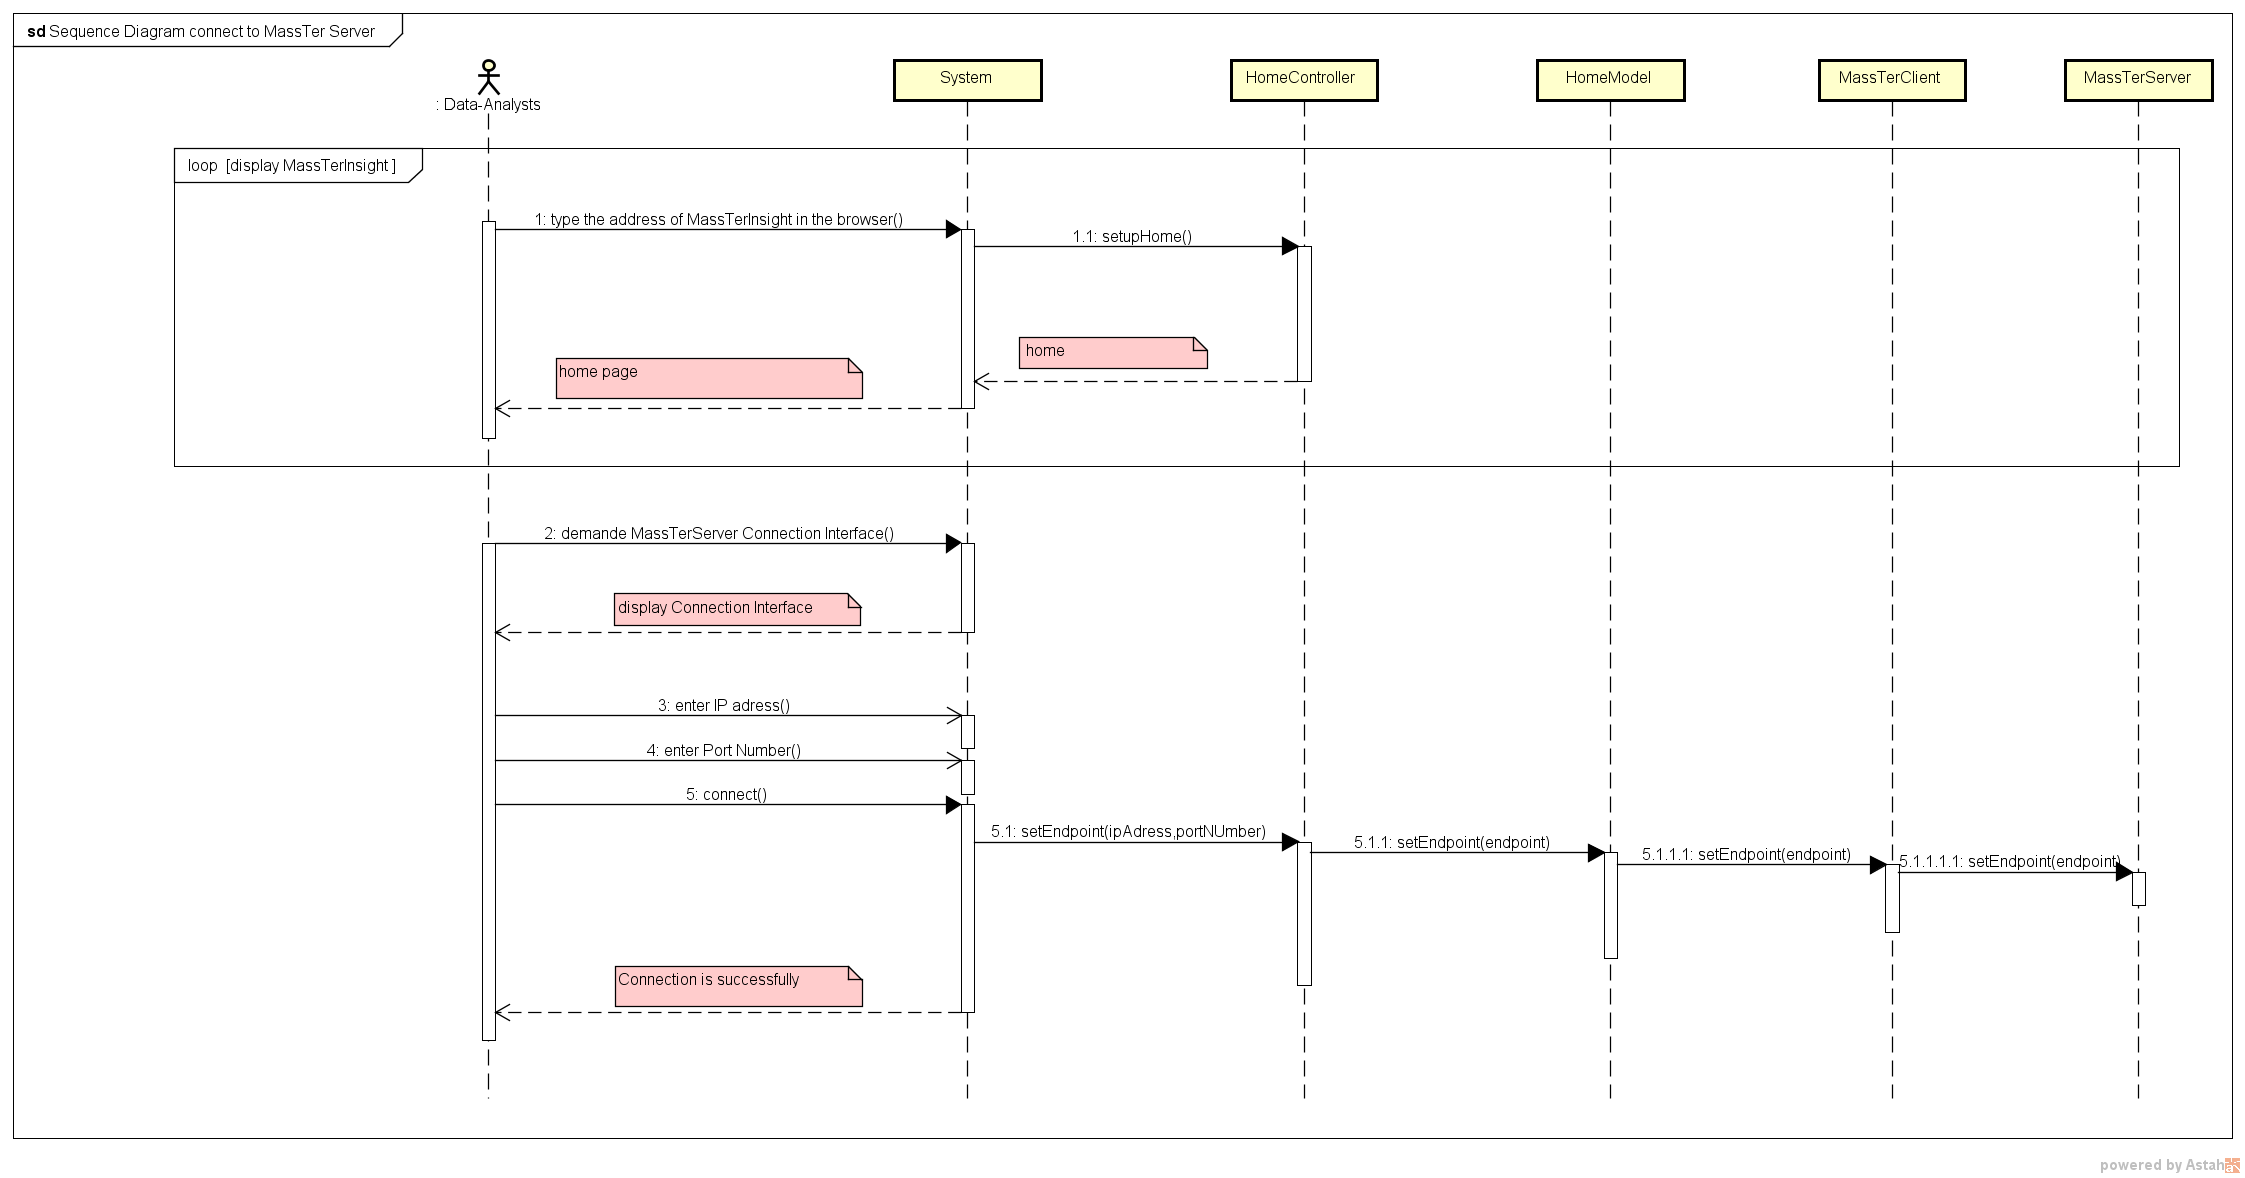
\includegraphics[width=1\textwidth]{SequenceDiagramconnectToMassTerServer.png}
		\caption{Sequence Diagram connect To MassTerServer}
	\end{figure}   
	
	\clearpage
	\newpage
	\subsubsection{Sequence Diagram use case ``consume web Service soap''}
	\clearpage
	\newpage
	\subsubsection{Sequence Diagram use case ``provide web Service soap''}
	\clearpage
	\newpage
	\subsubsection{Sequence Diagram use case ``load project''}
	\clearpage
	\newpage
	\subsubsection{Sequence Diagram use case ``display reports''}
	\clearpage
	\newpage
	\subsubsection{Sequence Diagram use case ``select report''}
	\clearpage
	\newpage
	\subsubsection{Sequence Diagram use case ``save report''}
	\clearpage
	\newpage
	\subsubsection{Sequence Diagram use case ``update settings''}
	\clearpage
	\newpage
	\subsubsection{Sequence Diagram use case ``run scenario''}
	\clearpage
	\newpage
	\section{Conclusion}
	Throughout this chapter, we have dissected the application to achieve gradually.
	We started by presenting the general architecture of the application, the we explained the global conception, unveiled through the packages diagrams, to go then to the detailed conception using class diagram, the sequences diagrams.  
	
	
\end{document}